
%% bare_conf.tex
%% V1.3
%% 2007/01/11
%% by Michael Shell
%% See:
%% http://www.michaelshell.org/
%% for current contact information.
%%
%% This is a skeleton file demonstrating the use of IEEEtran.cls
%% (requires IEEEtran.cls version 1.7 or later) with an IEEE conference paper.

%%
%% Support sites:
%% http://www.michaelshell.org/tex/ieeetran/
%% http://www.ctan.org/tex-archive/macros/latex/contrib/IEEEtran/
%% and
%% http://www.ieee.org/

%%*************************************************************************
%% Legal Notice:
%% This code is offered as-is without any warranty either expressed or
%% implied; without even the implied warranty of MERCHANTABILITY or
%% FITNESS FOR A PARTICULAR PURPOSE! 
%% User assumes all risk.
%% In no event shall IEEE or any contributor to this code be liable for
%% any damages or losses, including, but not limited to, incidental,
%% consequential, or any other damages, resulting from the use or misuse
%% of any information contained here.
%%
%% All comments are the opinions of their respective authors and are not
%% necessarily endorsed by the IEEE.
%%
%% This work is distributed under the LaTeX Project Public License (LPPL)
%% ( http://www.latex-project.org/ ) version 1.3, and may be freely used,
%% distributed and modified. A copy of the LPPL, version 1.3, is included
%% in the base LaTeX documentation of all distributions of LaTeX released
%% 2003/12/01 or later.
%% Retain all contribution notices and credits.
%% ** Modified files should be clearly indicated as such, including  **
%% ** renaming them and changing author support contact information. **
%%
%% File list of work: IEEEtran.cls, IEEEtran_HOWTO.pdf, bare_adv.tex,
%%                    bare_conf.tex, bare_jrnl.tex, bare_jrnl_compsoc.tex
%%*************************************************************************

% *** Authors should verify (and, if needed, correct) their LaTeX system  ***
% *** with the testflow diagnostic prior to trusting their LaTeX platform ***
% *** with production work. IEEE's font choices can trigger bugs that do  ***
% *** not appear when using other class files.                            ***
% The testflow support page is at:
% http://www.michaelshell.org/tex/testflow/



% Note that the a4paper option is mainly intended so that authors in
% countries using A4 can easily print to A4 and see how their papers will
% look in print - the typesetting of the document will not typically be
% affected with changes in paper size (but the bottom and side margins will).
% Use the testflow package mentioned above to verify correct handling of
% both paper sizes by the user's LaTeX system.
%
% Also note that the "draftcls" or "draftclsnofoot", not "draft", option
% should be used if it is desired that the figures are to be displayed in
% draft mode.
%
\documentclass[conference, letterpaper]{IEEEtran}
\usepackage{amsmath}
\usepackage{booktabs}
% Add the compsoc option for Computer Society conferences.
%
% If IEEEtran.cls has not been installed into the LaTeX system files,
% manually specify the path to it like:
% \documentclass[conference]{../sty/IEEEtran}





% Some very useful LaTeX packages include:
% (uncomment the ones you want to load)


% *** MISC UTILITY PACKAGES ***
%
%\usepackage{ifpdf}
% Heiko Oberdiek's ifpdf.sty is very useful if you need conditional
% compilation based on whether the output is pdf or dvi.
% usage:
% \ifpdf
%   % pdf code
% \else
%   % dvi code
% \fi
% The latest version of ifpdf.sty can be obtained from:
% http://www.ctan.org/tex-archive/macros/latex/contrib/oberdiek/
% Also, note that IEEEtran.cls V1.7 and later provides a builtin
% \ifCLASSINFOpdf conditional that works the same way.
% When switching from latex to pdflatex and vice-versa, the compiler may
% have to be run twice to clear warning/error messages.






% *** CITATION PACKAGES ***
%
%\usepackage{cite}
% cite.sty was written by Donald Arseneau
% V1.6 and later of IEEEtran pre-defines the format of the cite.sty package
% \cite{} output to follow that of IEEE. Loading the cite package will
% result in citation numbers being automatically sorted and properly
% "compressed/ranged". e.g., [1], [9], [2], [7], [5], [6] without using
% cite.sty will become [1], [2], [5]--[7], [9] using cite.sty. cite.sty's
% \cite will automatically add leading space, if needed. Use cite.sty's
% noadjust option (cite.sty V3.8 and later) if you want to turn this off.
% cite.sty is already installed on most LaTeX systems. Be sure and use
% version 4.0 (2003-05-27) and later if using hyperref.sty. cite.sty does
% not currently provide for hyperlinked citations.
% The latest version can be obtained at:
% http://www.ctan.org/tex-archive/macros/latex/contrib/cite/
% The documentation is contained in the cite.sty file itself.






% *** GRAPHICS RELATED PACKAGES ***
%
\ifCLASSINFOpdf
  % \usepackage[pdftex]{graphicx}
  % declare the path(s) where your graphic files are
  % \graphicspath{{../pdf/}{../jpeg/}}
  % and their extensions so you won't have to specify these with
  % every instance of \includegraphics
  % \DeclareGraphicsExtensions{.pdf,.jpeg,.png}
\else
  % or other class option (dvipsone, dvipdf, if not using dvips). graphicx
  % will default to the driver specified in the system graphics.cfg if no
  % driver is specified.
  % \usepackage[dvips]{graphicx}
  % declare the path(s) where your graphic files are
  % \graphicspath{{../eps/}}
  % and their extensions so you won't have to specify these with
  % every instance of \includegraphics
  % \DeclareGraphicsExtensions{.eps}
\fi
% graphicx was written by David Carlisle and Sebastian Rahtz. It is
% required if you want graphics, photos, etc. graphicx.sty is already
% installed on most LaTeX systems. The latest version and documentation can
% be obtained at: 
% http://www.ctan.org/tex-archive/macros/latex/required/graphics/
% Another good source of documentation is "Using Imported Graphics in
% LaTeX2e" by Keith Reckdahl which can be found as epslatex.ps or
% epslatex.pdf at: http://www.ctan.org/tex-archive/info/
%
% latex, and pdflatex in dvi mode, support graphics in encapsulated
% postscript (.eps) format. pdflatex in pdf mode supports graphics
% in .pdf, .jpeg, .png and .mps (metapost) formats. Users should ensure
% that all non-photo figures use a vector format (.eps, .pdf, .mps) and
% not a bitmapped formats (.jpeg, .png). IEEE frowns on bitmapped formats
% which can result in "jaggedy"/blurry rendering of lines and letters as
% well as large increases in file sizes.
%
% You can find documentation about the pdfTeX application at:
% http://www.tug.org/applications/pdftex





% *** MATH PACKAGES ***
%
%\usepackage[cmex10]{amsmath}
% A popular package from the American Mathematical Society that provides
% many useful and powerful commands for dealing with mathematics. If using
% it, be sure to load this package with the cmex10 option to ensure that
% only type 1 fonts will utilized at all point sizes. Without this option,
% it is possible that some math symbols, particularly those within
% footnotes, will be rendered in bitmap form which will result in a
% document that can not be IEEE Xplore compliant!
%
% Also, note that the amsmath package sets \interdisplaylinepenalty to 10000
% thus preventing page breaks from occurring within multiline equations. Use:
%\interdisplaylinepenalty=2500
% after loading amsmath to restore such page breaks as IEEEtran.cls normally
% does. amsmath.sty is already installed on most LaTeX systems. The latest
% version and documentation can be obtained at:
% http://www.ctan.org/tex-archive/macros/latex/required/amslatex/math/





% *** SPECIALIZED LIST PACKAGES ***
%
%\usepackage{algorithmic}
% algorithmic.sty was written by Peter Williams and Rogerio Brito.
% This package provides an algorithmic environment fo describing algorithms.
% You can use the algorithmic environment in-text or within a figure
% environment to provide for a floating algorithm. Do NOT use the algorithm
% floating environment provided by algorithm.sty (by the same authors) or
% algorithm2e.sty (by Christophe Fiorio) as IEEE does not use dedicated
% algorithm float types and packages that provide these will not provide
% correct IEEE style captions. The latest version and documentation of
% algorithmic.sty can be obtained at:
% http://www.ctan.org/tex-archive/macros/latex/contrib/algorithms/
% There is also a support site at:
% http://algorithms.berlios.de/index.html
% Also of interest may be the (relatively newer and more customizable)
% algorithmicx.sty package by Szasz Janos:
% http://www.ctan.org/tex-archive/macros/latex/contrib/algorithmicx/




% *** ALIGNMENT PACKAGES ***
%
%\usepackage{array}
% Frank Mittelbach's and David Carlisle's array.sty patches and improves
% the standard LaTeX2e array and tabular environments to provide better
% appearance and additional user controls. As the default LaTeX2e table
% generation code is lacking to the point of almost being broken with
% respect to the quality of the end results, all users are strongly
% advised to use an enhanced (at the very least that provided by array.sty)
% set of table tools. array.sty is already installed on most systems. The
% latest version and documentation can be obtained at:
% http://www.ctan.org/tex-archive/macros/latex/required/tools/


%\usepackage{mdwmath}
%\usepackage{mdwtab}
% Also highly recommended is Mark Wooding's extremely powerful MDW tools,
% especially mdwmath.sty and mdwtab.sty which are used to format equations
% and tables, respectively. The MDWtools set is already installed on most
% LaTeX systems. The lastest version and documentation is available at:
% http://www.ctan.org/tex-archive/macros/latex/contrib/mdwtools/


% IEEEtran contains the IEEEeqnarray family of commands that can be used to
% generate multiline equations as well as matrices, tables, etc., of high
% quality.


%\usepackage{eqparbox}
% Also of notable interest is Scott Pakin's eqparbox package for creating
% (automatically sized) equal width boxes - aka "natural width parboxes".
% Available at:
% http://www.ctan.org/tex-archive/macros/latex/contrib/eqparbox/





% *** SUBFIGURE PACKAGES ***
%\usepackage[tight,footnotesize]{subfigure}
% subfigure.sty was written by Steven Douglas Cochran. This package makes it
% easy to put subfigures in your figures. e.g., "Figure 1a and 1b". For IEEE
% work, it is a good idea to load it with the tight package option to reduce
% the amount of white space around the subfigures. subfigure.sty is already
% installed on most LaTeX systems. The latest version and documentation can
% be obtained at:
% http://www.ctan.org/tex-archive/obsolete/macros/latex/contrib/subfigure/
% subfigure.sty has been superceeded by subfig.sty.



%\usepackage[caption=false]{caption}
%\usepackage[font=footnotesize]{subfig}
% subfig.sty, also written by Steven Douglas Cochran, is the modern
% replacement for subfigure.sty. However, subfig.sty requires and
% automatically loads Axel Sommerfeldt's caption.sty which will override
% IEEEtran.cls handling of captions and this will result in nonIEEE style
% figure/table captions. To prevent this problem, be sure and preload
% caption.sty with its "caption=false" package option. This is will preserve
% IEEEtran.cls handing of captions. Version 1.3 (2005/06/28) and later 
% (recommended due to many improvements over 1.2) of subfig.sty supports
% the caption=false option directly:
%\usepackage[caption=false,font=footnotesize]{subfig}
%
% The latest version and documentation can be obtained at:
% http://www.ctan.org/tex-archive/macros/latex/contrib/subfig/
% The latest version and documentation of caption.sty can be obtained at:
% http://www.ctan.org/tex-archive/macros/latex/contrib/caption/




% *** FLOAT PACKAGES ***
%
%\usepackage{fixltx2e}
% fixltx2e, the successor to the earlier fix2col.sty, was written by
% Frank Mittelbach and David Carlisle. This package corrects a few problems
% in the LaTeX2e kernel, the most notable of which is that in current
% LaTeX2e releases, the ordering of single and double column floats is not
% guaranteed to be preserved. Thus, an unpatched LaTeX2e can allow a
% single column figure to be placed prior to an earlier double column
% figure. The latest version and documentation can be found at:
% http://www.ctan.org/tex-archive/macros/latex/base/



%\usepackage{stfloats}
% stfloats.sty was written by Sigitas Tolusis. This package gives LaTeX2e
% the ability to do double column floats at the bottom of the page as well
% as the top. (e.g., "\begin{figure*}[!b]" is not normally possible in
% LaTeX2e). It also provides a command:
%\fnbelowfloat
% to enable the placement of footnotes below bottom floats (the standard
% LaTeX2e kernel puts them above bottom floats). This is an invasive package
% which rewrites many portions of the LaTeX2e float routines. It may not work
% with other packages that modify the LaTeX2e float routines. The latest
% version and documentation can be obtained at:
% http://www.ctan.org/tex-archive/macros/latex/contrib/sttools/
% Documentation is contained in the stfloats.sty comments as well as in the
% presfull.pdf file. Do not use the stfloats baselinefloat ability as IEEE
% does not allow \baselineskip to stretch. Authors submitting work to the
% IEEE should note that IEEE rarely uses double column equations and
% that authors should try to avoid such use. Do not be tempted to use the
% cuted.sty or midfloat.sty packages (also by Sigitas Tolusis) as IEEE does
% not format its papers in such ways.





% *** PDF, URL AND HYPERLINK PACKAGES ***
%
%\usepackage{url}
% url.sty was written by Donald Arseneau. It provides better support for
% handling and breaking URLs. url.sty is already installed on most LaTeX
% systems. The latest version can be obtained at:
% http://www.ctan.org/tex-archive/macros/latex/contrib/misc/
% Read the url.sty source comments for usage information. Basically,
% \url{my_url_here}.





% *** Do not adjust lengths that control margins, column widths, etc. ***
% *** Do not use packages that alter fonts (such as pslatex).         ***
% There should be no need to do such things with IEEEtran.cls V1.6 and later.
% (Unless specifically asked to do so by the journal or conference you plan
% to submit to, of course. )


% correct bad hyphenation here
\hyphenation{op-tical net-works semi-conduc-tor}

% *** GRAPHICS RELATED PACKAGES ***
%
\ifCLASSINFOpdf
   \usepackage[pdftex]{graphicx}
   \usepackage{subcaption}
   \usepackage[export]{adjustbox}
\else
\fi

\usepackage{algorithm}
\usepackage{algpseudocode}

% *** MATH PACKAGES ***
%
\usepackage{color}
%
\usepackage{fancyhdr}
\usepackage[caption=false,font=footnotesize]{subfig}
\usepackage{booktabs}
\usepackage{array}
\usepackage{amssymb}
\usepackage{amsfonts}
\usepackage{float}

\renewcommand{\thispagestyle}[2]{} 


\fancypagestyle{plain}{
        \fancyhead{}
        \fancyhead[C]{first page center header}
        \fancyfoot{}
        \fancyfoot[C]{first page center footer}
}
\pagestyle{fancy}


\headheight 20pt
\footskip 20pt

\rhead{}

%Enter the first page number of your paper below
\setcounter{page}{1}

%Header
\fancyhead[R]{\textit{(IJACSA) International Journal of Advanced Computer Science and Applications, \\ Vol. XXX, No. XXX, 2024}}
\renewcommand{\headrulewidth}{0pt}

%Footer
\fancyfoot[C]{www.ijacsa.thesai.org}
\renewcommand{\footrulewidth}{0.5pt}
\fancyfoot[R]{\thepage \  $|$ P a g e }


\begin{document}

%
% paper title
% can use linebreaks \\ within to get better formatting as desired
\title{Análisis de sentimientos y favorabilidad política en comentarios de Youtube durante las elecciones 
presidenciales peruanas de 2026}


% author names and affiliations
% use a multiple column layout for up to three different
% affiliations
\makeatletter
\newcommand{\linebreakand}{
  \end{@IEEEauthorhalign}
  \hfill\mbox{}\par
  \mbox{}\hfill\begin{@IEEEauthorhalign}
}
\makeatother
\author{
    Jose Alva Cornejo
    % ,Esdras D. Vasquez, Jose Calizaya Quispe, Roxana Flores-Quispe, Yuber Velazco-Paredes\\
    Universidad Nacional de San Agustín de Arequipa, Arequipa, Perú\\
    %Emails: jalvac@unsa.edu.pe, ediazva@unsa.edu.pe, jcalizayaq@unsa.edu.pe, \\rfloresqu@unsa.edu.pe, yvelazco@unsa.edu.pe
}




% conference papers do not typically use \thanks and this command
% is locked out in conference mode. If really needed, such as for
% the acknowledgment of grants, issue a \IEEEoverridecommandlockouts
% after \documentclass

% for over three affiliations, or if they all won't fit within the width
% of the page, use this alternative format:
% 
%\author{\IEEEauthorblockN{Michael Shell\IEEEauthorrefmark{1},
%Homer Simpson\IEEEauthorrefmark{2},
%James Kirk\IEEEauthorrefmark{3}, 
%Montgomery Scott\IEEEauthorrefmark{3} and
%Eldon Tyrell\IEEEauthorrefmark{4}}
%\IEEEauthorblockA{\IEEEauthorrefmark{1}School of Electrical and Computer Engineering\\
%Georgia Institute of Technology,
%Atlanta, Georgia 30332--0250\\ Email: see http://www.michaelshell.org/contact.html}
%\IEEEauthorblockA{\IEEEauthorrefmark{2}Twentieth Century Fox, Springfield, USA\\
%Email: homer@thesimpsons.com}
%\IEEEauthorblockA{\IEEEauthorrefmark{3}Starfleet Academy, San Francisco, California 96678-2391\\
%Telephone: (800) 555--1212, Fax: (888) 555--1212}
%\IEEEauthorblockA{\IEEEauthorrefmark{4}Tyrell Inc., 123 Replicant Street, Los Angeles, California 90210--4321}}




% use for special paper notices
%\IEEEspecialpapernotice{(Invited Paper)}


% make the title area
\maketitle


\begin{abstract}
La creciente actividad política en redes sociales ha generado grandes volúmenes de contenido textual, dificultando el análisis de la opinión y el sentimiento político mediante métodos tradicionales. Para abordar este problema, se emplearon técnicas de procesamiento del lenguaje natural y aprendizaje profundo, utilizando un modelo basado en la arquitectura RoBERTa especializado en lenguaje de redes sociales en español. En este trabajo se propone un enfoque para clasificar sentimientos políticos en comentarios de redes sociales durante la segunda vuelta de las elecciones presidenciales peruanas de 2026. Se recopilaron 2743 comentarios de TikTok asociados a los candidatos de los dos partidos políticos en contienda; % (JP y K) 
ademas de contenido neutral, los cuales fueron clasificados mediante RoBERTuito. A partir de las predicciones se calcularon indicadores de favorabilidad neta y ponderada, además de métricas relacionadas con la confianza del modelo, participación de los usuarios y nivel de \textit{engagement}. Los resultados muestran una favorabilidad neta positiva y de magnitud similar para ambos candidatos, en contraste con una favorabilidad levemente negativa en las publicaciones neutrales, comportamiento consistente con un posible escenario de \textit{echo chamber}. Sin embargo, la baja recurrencia de los usuarios y la escasa interacción entre categorías políticas impidieron calcular una medida de polarización afectiva individual, limitando los resultados a una medida de favorabilidad agregada.
\end{abstract}

% IEEEtran.cls defaults to using nonbold math in the Abstract.
% This preserves the distinction between vectors and scalars. However,
% if the conference you are submitting to favors bold math in the abstract,
% then you can use LaTeX's standard command \boldmath at the very start
% of the abstract to achieve this. Many IEEE journals/conferences frown on
% math in the abstract anyway.

% no keywords


\begin{IEEEkeywords}
Sentiment Analysis, Natural Language Processing, Deep Learning, Transformer Models, Slang, Social Media, Political Opinion Mining.
\end{IEEEkeywords}


% For peer review papers, you can put extra information on the cover
% page as needed:
% \ifCLASSOPTIONpeerreview
% \begin{center} \bfseries EDICS Category: 3-BBND \end{center}
% \fi
%
% For peerreview papers, this IEEEtran command inserts a page break and
% creates the second title. It will be ignored for other modes.
\IEEEpeerreviewmaketitle



\section{Introducción}

Las redes sociales se han consolidado como uno de los principales espacios para la discusión política y la expresión de opiniones ciudadanas. Plataformas como Facebook, Instagram y TikTok permiten que millones de usuarios compartan publicaciones, comentarios e interacciones relacionadas con acontecimientos políticos, generando grandes volúmenes de información que reflejan la percepción pública sobre candidatos, partidos y políticas gubernamentales \cite{statista2026} \cite{statista_tiktok2026}. Debido a su alcance e influencia, estas plataformas constituyen una fuente relevante para estudiar el comportamiento político y las tendencias de opinión mediante técnicas de procesamiento del lenguaje natural (Natural Language Processing, NLP) \cite{ref1}. Además, la interacción con contenido político en redes sociales se ha relacionado con cambios en las actitudes políticas de los usuarios. Afyare \cite{afyare2025socialmedia} encontró que un mayor nivel de involucramiento con contenido político se correlaciona con opiniones más polarizadas, destacando que estas plataformas pueden funcionar tanto como herramientas de movilización política como canales para la propagación de desinformación. En este contexto, el análisis automático del contenido generado por los usuarios constituye una alternativa para estudiar la dinámica de la opinión pública durante procesos electorales.

Una de las principales soluciones empleadas para este problema es el análisis automático de sentimientos, mediante el cual se identifica la polaridad expresada en un texto y se clasifica generalmente como positiva, negativa o neutra. Esta aproximación permite analizar grandes volúmenes de publicaciones y comentarios sin depender exclusivamente de métodos tradicionales como las encuestas. En particular, los avances en aprendizaje profundo y en modelos basados en la arquitectura Transformer han permitido mejorar el desempeño de las tareas de clasificación textual al capturar relaciones contextuales complejas presentes en el lenguaje natural. Modelos como BERT y sus variantes han demostrado resultados competitivos en diversas aplicaciones de análisis de sentimientos \cite{Singh2026}.

Estas técnicas también han sido aplicadas específicamente al análisis de sentimientos y polarización política. Martínez-España et al. \cite{polariz} propusieron una metodología basada en modelos Transformer para medir la polarización afectiva a partir de publicaciones en redes sociales. De manera similar, Bor et al. \cite{bor2023} utilizaron análisis de sentimientos para cuantificar la polarización política en Twitter considerando diferentes grupos políticos y políticas públicas. En el contexto peruano, Ayma et al. \cite{Ayma2024} emplearon representaciones textuales como TF-IDF y Word2Vec junto con modelos tradicionales de aprendizaje automático para analizar mensajes publicados durante las elecciones presidenciales de 2021. Asimismo, Carrera et al. \cite{Carrera2026} compararon técnicas tradicionales con modelos basados en Transformers para clasificar comentarios relacionados con proyectos de ley peruanos, obteniendo mejores resultados mediante arquitecturas profundas. Estos trabajos muestran que tanto los métodos tradicionales de representación textual como los modelos Transformer constituyen alternativas para abordar la clasificación de sentimientos políticos.

Sin embargo, una limitación de estos enfoques es que muchos modelos son entrenados sobre corpus generales y pueden no representar adecuadamente las características lingüísticas presentes en determinados dominios o regiones. En el caso del español utilizado en redes sociales peruanas, son frecuentes las expresiones coloquiales, la jerga, el sarcasmo, las abreviaturas y otras construcciones propias de la comunicación informal. El uso de modelos generales que no consideran estas características puede afectar su capacidad para clasificar correctamente el sentimiento en este tipo de contenido \cite{10.1145/3446132.3446424} \cite{robertuito}. Además, gran parte de la literatura existente se concentra en Twitter/X y en contextos internacionales, mientras que otras plataformas con una elevada actividad política, como Facebook, Instagram y TikTok, han recibido una atención comparativamente menor \cite{limaretail2026}.

Como alternativa a los modelos generales, se han desarrollado modelos especializados en el lenguaje de redes sociales. Entre ellos destaca RoBERTuito, un modelo basado en la arquitectura RoBERTa y preentrenado sobre más de 500 millones de publicaciones en español provenientes de redes sociales. Su entrenamiento sobre este tipo de contenido permite representar características propias del lenguaje informal utilizado en estas plataformas. Además, estudios orientados específicamente al español peruano han mostrado que el ajuste de modelos de este tipo puede mejorar el desempeño en tareas de análisis de sentimientos al incorporar vocabulario y expresiones características del contexto nacional \cite{CalizayaMilla2026}.

En este trabajo se propone un enfoque basado en aprendizaje profundo para analizar el sentimiento político expresado en contenido textual de redes sociales durante la segunda vuelta de las elecciones presidenciales peruanas de 2026. Para ello, se construye un conjunto de datos a partir de comentarios obtenidos de publicaciones relacionadas con los dos candidatos en contienda y con contenido de carácter neutral. Posteriormente, los comentarios son clasificados mediante RoBERTuito y, a partir de sus predicciones, se calculan métricas de favorabilidad neta y ponderada, incorporando además información relacionada con la participación de los usuarios y el nivel de \textit{engagement}. El enfoque se inspira en la metodología de Martínez-España et al. \cite{polariz}, pero se adapta a las características y limitaciones del conjunto de datos disponible.
%%puede precisar la diferencia con Martinez

El resto del artículo se organiza de la siguiente manera. La Sección II presenta el estado del arte relacionado con el análisis de sentimientos, el análisis de polarización política y los modelos aplicados al contexto peruano. La Sección III describe el método propuesto, incluyendo la obtención y el preprocesamiento de los datos, la clasificación de sentimientos y las métricas utilizadas para el análisis. La Sección IV presenta los resultados obtenidos y su interpretación. Finalmente, la Sección V expone las conclusiones y las posibles líneas de trabajo futuro.

\section{Estado del Arte}
El análisis de sentimientos aplicado al ámbito político ha adquirido una creciente relevancia debido al incremento del contenido generado por usuarios en redes sociales y a la disponibilidad de técnicas avanzadas de procesamiento del lenguaje natural. Las investigaciones recientes han abordado este problema desde diferentes perspectivas, incluyendo el estudio de la polarización política, la clasificación automática de opiniones y el desarrollo de modelos especializados para lenguaje informal.

Una de las principales líneas de investigación corresponde al análisis de la polarización política mediante técnicas de análisis de sentimientos. Martínez-España et al. \cite{polariz} propusieron una metodología para medir la polarización afectiva individual utilizando modelos basados en Transformers sobre datos obtenidos de redes sociales. Su trabajo demostró que el análisis automático de sentimientos constituye una alternativa viable a los métodos tradicionales basados en encuestas para estudiar el comportamiento político. De forma similar, Bor et al. \cite{bor2023} emplearon análisis de sentimientos para cuantificar la polarización política en Twitter considerando distintos grupos políticos y diversas políticas públicas en Estados Unidos, evidenciando diferencias significativas en los niveles de polarización según el tema analizado.

Otra línea de investigación se ha enfocado en la clasificación automática de sentimientos políticos utilizando técnicas de aprendizaje automático y aprendizaje profundo. En el contexto peruano, Ayma et al. \cite{Ayma2024} analizaron mensajes publicados en Twitter/X durante las elecciones presidenciales de 2021 empleando representaciones textuales como TF-IDF y Word2Vec en combinación con algoritmos tradicionales de clasificación, obteniendo valores de F1-score superiores a 0.93. Posteriormente, Carrera et al. \cite{Carrera2026} compararon representaciones textuales tradicionales y modelos basados en Transformers para clasificar comentarios relacionados con proyectos de ley peruanos. Sus resultados mostraron que los modelos Transformer superaron consistentemente a los enfoques clásicos, alcanzando precisiones superiores al 88\%.

Pandey et al. \cite{pandey2025twitter} analizaron el sentimiento de los votantes durante las elecciones legislativas de Bihar de 2025 utilizando más de 1\,100 publicaciones obtenidas mediante la API de Twitter. Los autores compararon tres métodos de clasificación de sentimientos: Random Forest, Support Vector Machine (SVM) y el modelo basado en transformadores BERT. Inicialmente, las publicaciones fueron etiquetadas utilizando VADER y posteriormente se evaluaron las tendencias de cada partido político mediante el \textit{Net Sentiment Score} (NSS). Los resultados mostraron que BERT obtuvo una exactitud del 80\%, superando a los modelos tradicionales y evidenciando la capacidad de los modelos basados en transformadores para realizar análisis de sentimientos en escenarios electorales con conjuntos de datos de tamaño reducido.

% Chire Saire y Vilca Zuñiga \cite{chire2021analysis} analizaron la reacción de los usuarios de Twitter ante el proceso de vacancia presidencial ocurrido en Perú durante la pandemia por COVID-19. El estudio tuvo como objetivo identificar los principales temas de discusión y evaluar el impacto que la crisis política generó en la población peruana a partir de las publicaciones realizadas en esta red social. Los autores recopilaron mensajes relacionados con el proceso de destitución presidencial y realizaron un análisis de las opiniones expresadas por los usuarios para identificar tendencias en el debate político. Los resultados evidenciaron que Twitter constituyó una fuente relevante para analizar la percepción ciudadana y la reacción de la población frente a los acontecimientos políticos ocurridos durante dicho periodo.

Rizk et al. \cite{rizk2023predicting} propusieron un modelo para predecir los resultados de las elecciones presidenciales de Estados Unidos de 2020 utilizando publicaciones geolocalizadas de Twitter. La metodología combinó análisis de sentimientos, un clasificador Multinomial Naive Bayes y técnicas de aprendizaje automático para estimar tanto el voto popular como los votos del colegio electoral en los 50 estados. Además, los autores eliminaron publicaciones generadas por bots y valores atípicos, analizaron la evolución temporal y espacial de la opinión pública, y emplearon análisis de redes y detección de comunidades para identificar patrones de interacción entre los usuarios. Los resultados mostraron que el modelo predijo correctamente la victoria de Joe Biden, alcanzando una concordancia del 89.9\% con los resultados oficiales de las elecciones.

Rodríguez-Ibáñez et al. \cite{rodriguez2021sentiment} realizaron un estudio sobre el análisis de sentimientos en publicaciones de Twitter relacionadas con las elecciones presidenciales españolas de 2019. Los autores recopilaron miles de publicaciones realizadas antes y después del proceso electoral y propusieron una metodología basada en dos etapas: una caracterización estadística utilizando métricas como entropía, información mutua y el \textit{Compounded Aggregated Positivity Index} (CAPI), seguida de la extracción de características mediante técnicas de aprendizaje no lineal, incluyendo autoencoders y métodos de incrustación estocástica. Los resultados mostraron que tanto las métricas estadísticas como las representaciones obtenidas permitieron caracterizar la evolución temporal del sentimiento y evidenciar diferencias en la polaridad entre los distintos partidos políticos y sus líderes durante el periodo electoral.

Chaudhry et al. \cite{chaudhry2022sentiment} realizaron un análisis de sentimientos sobre publicaciones de Twitter relacionadas con las elecciones presidenciales de Estados Unidos de 2020, considerando el periodo previo, durante y posterior a los comicios. Para ello, construyeron un conjunto de datos utilizando la API de Twitter, aplicaron técnicas de preprocesamiento y extracción de características mediante TF-IDF, y emplearon un clasificador Naive Bayes para determinar la polaridad de los mensajes. Los autores compararon los resultados obtenidos con los resultados oficiales de las elecciones y analizaron el comportamiento de los estados disputados y de aquellos considerados atípicos. Los experimentos mostraron que el sentimiento expresado en Twitter coincidió con los resultados electorales en la mayoría de los casos, además de evidenciar cambios en la opinión pública antes y después de las elecciones. El clasificador alcanzó una exactitud del 94.58\% y una precisión del 93.19\%.

En conjunto, estos trabajos evidencian el potencial de los modelos basados en Transformers para el análisis de sentimientos políticos. Sin embargo, la mayoría de las investigaciones se ha desarrollado utilizando datos provenientes de Twitter/X o en contextos distintos al peruano. Asimismo, existe un número limitado de estudios que empleen publicaciones y comentarios obtenidos de Facebook e Instagram, plataformas que concentran una elevada actividad política y presentan características lingüísticas propias del lenguaje informal utilizado por los usuarios peruanos.

En este contexto, el presente trabajo propone evaluar modelos de aprendizaje profundo para la clasificación de sentimientos políticos utilizando contenido textual obtenido de tanto Facebook, Instagram y TikTok en el idioma español. De esta manera, se busca contribuir al desarrollo de modelos adaptados al contexto peruano y ampliar la evidencia existente sobre el análisis de sentimientos en plataformas que han recibido menor atención dentro de la literatura especializada.

\section{Método Propuesto}

\begin{figure}
    \centering
    \includegraphics[width=0.85\linewidth]{pipeline_3.png}
    \caption{Pipeline}
    \label{fig:metodo}
\end{figure}

La figura \ref{fig:metodo} muestra una representación visual del método usado, con el fin de poder obtener cierta medición de polarización política en el dataset utilizado.

\subsection{Obtención de datos crudos}

Con el objetivo de construir un conjunto de datos inicial para el análisis de sentimientos políticos, y teniendo en cuenta el porcentaje de uso de redes sociales en Perú y las restricciones recientes de acceso a datos en plataformas como Facebook y Twitter/X \cite{ANTONAKAKI2021114006}, se decidió utilizar datos provenientes de TikTok. Se recopiló un total de 2743 comentarios mediante técnicas de \textit{web scraping}, centrados en publicaciones relacionadas con la segunda vuelta de las elecciones presidenciales peruanas, celebradas el 7 de junio de 2026.

Las publicaciones fueron clasificadas en tres categorías: \textit{JP}, \textit{K} y \textit{neutral}. Las dos primeras representan a cada uno de los candidatos presidenciales participantes en la segunda vuelta, mientras que \textit{neutral} agrupa publicaciones de carácter informativo, principalmente relacionadas con el conteo rápido de votos durante las horas posteriores al cierre de la jornada electoral. La selección de publicaciones priorizó aquellas con mayor cantidad de comentarios, con el fin de aumentar el volumen y la diversidad de opiniones recopiladas.

\subsection{Preprocesado}

Durante el preprocesamiento se extrajeron únicamente los atributos necesarios para el análisis: contenido textual, identificador y nombre del usuario, cantidad de \textit{likes}, identificador del comentario y de la publicación, así como la información necesaria para determinar si el comentario correspondía a una respuesta a otro (comentario padre). Adicionalmente, cada comentario fue etiquetado con la categoría de la publicación de origen (\textit{party}: \textit{JP}, \textit{K} o \textit{neutral}). Finalmente, los datos de todas las publicaciones fueron unificados en un único conjunto de datos estructurado, según se describe en el Algoritmo~\ref{alg:preprocess}.

\begin{algorithm}[H]
\caption{Preprocesamiento y unificación de los comentarios recolectados}
\label{alg:preprocess}
\begin{algorithmic}[1]
\Require Archivos de comentarios obtenidos mediante \textit{web scraping}, cada uno asociado a una categoría política.
\Ensure Conjunto de datos unificado y etiquetado.
\ForAll{archivo de comentarios}
    \State Extraer texto, identificadores (usuario, comentario, publicación), \textit{likes} e identificador de respuesta.
    \State Determinar si el comentario es una respuesta y registrar su comentario padre.
    \State Asignar la etiqueta política según el origen del archivo.
\EndFor
\State \Return Conjunto de datos unificado.
\end{algorithmic}
\end{algorithm}

\begin{figure}[H]
    \centering
    \includegraphics[width=1\linewidth]{preprocesado.png}
    \caption{Datos preparados para input de modelo}
    \label{fig:placeholder}
\end{figure}

\subsection{Clasificación de sentimiento}

Cada comentario preprocesado fue clasificado utilizando \textit{RoBERTuito}, una variante de RoBERTa entrenada con publicaciones de redes sociales escritas por usuarios peruanos, lo que le permite capturar expresiones coloquiales y variaciones lingüísticas propias del contexto nacional. Para cada comentario $c_i$, el modelo produce una etiqueta de sentimiento $S_i \in \{\text{negative},\ \text{neutral},\ \text{positive}\}$ y un puntaje de confianza $P_i \in [0,1]$, de forma que

\begin{equation}
(S_i,P_i)=f_{\mathrm{RoBERTuito}}(c_i).
\end{equation}

Ambos valores fueron incorporados al conjunto de datos para su uso posterior en el análisis de polarización.

\subsection{Análisis de polarización}

Con el propósito de cuantificar la polarización política presente en los comentarios recopilados, se definieron diversas métricas basadas en los resultados de la clasificación de sentimientos. En una primera etapa se empleó el \textit{Net Sentiment Score} (NSS), utilizado por Pandey et al. \cite{pandey2025twitter} para evaluar la tendencia del sentimiento hacia distintos partidos políticos durante las elecciones de Bihar de 2025, junto con una variante ponderada por la confianza del modelo. En una segunda etapa se buscó replicar, de forma adaptada, el indicador de polarización afectiva individual propuesto por Martínez-España et al. \cite{polariz}.

\subsubsection{Favorabilidad neta y ponderada}

Para cada categoría política se contabilizó el número de comentarios positivos ($N_{pos}$), negativos ($N_{neg}$) y neutrales ($N_{neu}$), con $N=N_{pos}+N_{neg}+N_{neu}$, y se calculó la favorabilidad neta (NSS) como

\begin{equation}
F_{\mathrm{neta}} = \frac{N_{pos}-N_{neg}}{N} \in [-1,1].
\label{eq:favorabilidad_neta}
\end{equation}

Para incorporar la confianza del modelo, a cada comentario se le asignó un valor $s_i \in \{1,0,-1\}$ según su sentimiento (positivo, neutral, negativo), y su aporte individual se definió como $a_i = s_i P_i$, donde $P_i$ es la confianza entregada por el modelo. La favorabilidad ponderada para cada categoría se obtuvo mediante

\begin{equation}
F_{\mathrm{pond}} = \frac{1}{N}\sum_{i=1}^{N} s_i P_i.
\label{eq:favorabilidad_ponderada}
\end{equation}

De esta manera, las clasificaciones con mayor confianza tienen una influencia proporcionalmente mayor en la métrica final.

\subsubsection{Indicador de polarización afectiva individual}
\label{subsubsec:ap_individual}

A diferencia de las métricas anteriores, que se calculan de forma agregada por categoría, este indicador busca cuantificar la polarización a nivel de cada usuario, siguiendo la formulación de Martínez-España et al. \cite{polariz}. Para ello es necesario, en primer lugar, determinar el grupo de afinidad política (\textit{ingroup}) de cada usuario.

Para cada usuario $i$, se contabilizó el número de interacciones positivas ($\text{Pos}_{i,j}$) y negativas ($\text{Neg}_{i,j}$) hacia cada categoría política $j$. El \textit{ingroup} se determinó como la categoría con la mayor cantidad de interacciones positivas:

\begin{equation}
\text{Ingroup}(i) = \operatorname*{argmax}_{j}\left(\text{Pos}_{i,j}\right).
\label{eq:ingroup}
\end{equation}

En caso de que un usuario no registre interacciones positivas con ninguna categoría, o exista un empate entre dos o más categorías, el usuario se clasifica como \textit{Undetermined}, es decir, sin afinidad política clara.

A partir del \textit{ingroup} determinado, se calculó la polarización afectiva hacia el propio grupo ($\mathrm{AP_{In}}$) y hacia el resto de las categorías ($\mathrm{AP_{Out}}$):

\begin{equation}
\mathrm{AP}(i)_{\mathrm{In}} = \text{Pos}_{i,j} - \text{Neg}_{i,j}, \qquad j=\text{Ingroup}(i),
\label{eq:ap_in}
\end{equation}

\begin{equation}
\mathrm{AP}(i)_{\mathrm{Out}} = \sum_{j' \neq j}\left(\text{Pos}_{i,j'} - \text{Neg}_{i,j'}\right).
\label{eq:ap_out}
\end{equation}

Finalmente, la polarización afectiva individual se obtuvo como la diferencia entre ambas componentes:

\begin{equation}
\mathrm{AP}(i) = \mathrm{AP}(i)_{\mathrm{In}} - \mathrm{AP}(i)_{\mathrm{Out}}.
\label{eq:ap_final}
\end{equation}

Dado que $\mathrm{AP}(i)$ depende del volumen total de interacción de cada usuario, se calculó adicionalmente una versión normalizada (\textit{spread}), adaptada de la propuesta de Wagner \cite{wagner2021affective}:

\begin{equation}
\mathrm{spread}(i) = \sqrt{\frac{\sum_{j}\left(\text{Pos}_{i,j}-\text{Neg}_{i,j}\right)^2}{n_i}},
\label{eq:spread}
\end{equation}

donde $n_i$ representa el número total de interacciones del usuario $i$ en todas las categorías consideradas.

Tanto $\mathrm{AP}(i)$ como $\mathrm{spread}(i)$ fueron posteriormente clasificados en tres niveles (bajo, medio y alto), utilizando como referencia la media y la desviación estándar de cada indicador, siguiendo el mismo criterio empleado en \cite{polariz}.

Cabe señalar que la categoría \textit{neutral} fue considerada como una categoría válida dentro del conjunto de posibles \textit{ingroups} y como parte del cálculo de $\mathrm{AP_{Out}}$, en lugar de excluirse del análisis. Esta decisión responde al estado actual del conjunto de datos, compuesto mayoritariamente por publicaciones de carácter neutral, y se retoma como parte de la discusión metodológica en la Sección~\ref{sec:resultados}, donde también se abordan las implicaciones de este tratamiento sobre la interpretación del indicador.

\begin{algorithm}[H]
\caption{Cálculo de métricas de polarización}
\begin{algorithmic}[1]
\Require Conjunto de comentarios clasificados.

\ForAll{categoría política}
    \State Calcular favorabilidad neta y ponderada (Ecuaciones~\ref{eq:favorabilidad_neta}--\ref{eq:favorabilidad_ponderada}).
\EndFor

\ForAll{usuario}
    \State Calcular $\text{Pos}_{i,j}$ y $\text{Neg}_{i,j}$ para cada categoría $j$.
    \State Determinar el \textit{ingroup} (Ecuación~\ref{eq:ingroup}).
    \If{\textit{ingroup} distinto de \textit{Undetermined}}
        \State Calcular $\mathrm{AP_{In}}$, $\mathrm{AP_{Out}}$, $\mathrm{AP}$ y \textit{spread} (Ecuaciones~\ref{eq:ap_in}--\ref{eq:spread}).
        \State Clasificar $\mathrm{AP}$ y \textit{spread} en niveles (bajo/medio/alto).
    \EndIf
\EndFor

\State Generar datos a ser ploteados.
\end{algorithmic}
\end{algorithm}

\section{Resultados e interpretación}

Esta sección presenta los resultados de la clasificación de sentimiento y de
las métricas calculadas sobre $552{,}456$ comentarios de videos publicados por
fuentes agrupadas como izquierda, derecha y neutral. La etiqueta \textit{party}
identifica el grupo asignado a la fuente del video; no representa una etiqueta
de sentimiento ni una clasificación política del autor del comentario.

\subsection{Distribución de sentimiento y favorabilidad}

La Tabla~\ref{tab:sentimiento_favorabilidad} resume el número de comentarios,
la distribución de sentimiento y las medidas de favorabilidad por grupo de
fuentes. La favorabilidad neta corresponde a la diferencia entre las
proporciones de comentarios positivos y negativos. La medida ponderada
normalizada incorpora los puntajes de confianza del modelo.

\begin{table}[H]
\centering
\caption{Sentimiento predicho y favorabilidad por grupo de fuentes.}
\label{tab:sentimiento_favorabilidad}
\begin{tabular}{lrrr}
\hline
Métrica & Derecha & Izquierda & Neutral \\
\hline
Comentarios & 116{,}111 & 264{,}520 & 171{,}825 \\
Negativo (\%) & 49.34 & 51.74 & 61.43 \\
Neutro (\%) & 35.10 & 30.13 & 28.13 \\
Positivo (\%) & 15.56 & 18.13 & 10.44 \\
Favorabilidad neta & $-0.338$ & $-0.336$ & $-0.510$ \\
Ponderada norm. & $-0.281$ & $-0.282$ & $-0.422$ \\
\hline
\end{tabular}
\end{table}

En los tres grupos, el sentimiento negativo es la clase más frecuente. Las
favorabilidades netas de las fuentes de derecha e izquierda son prácticamente
iguales ($-0.338$ y $-0.336$), mientras que el grupo neutral registra un valor
más negativo ($-0.510$). La medida ponderada presenta el mismo orden. Estas
diferencias describen la valencia general predicha en los comentarios
recolectados; no demuestran que los comentarios estén dirigidos al grupo
político asociado al canal ni que sus autores apoyen o rechacen ese grupo.

\subsection{Polarización afectiva individual y \textit{spread}}

El análisis individual incluyó $135{,}259$ usuarios con al menos un comentario
positivo o negativo. De ellos, $100{,}870$ ($74.58\%$) quedaron como
\textit{Undetermined}: no tuvieron comentarios positivos en los grupos
políticos considerados o empataron en su máximo. Por tanto, $34{,}389$ usuarios
tuvieron un grupo de afinidad operacional determinado. Esta asignación se basa
en el grupo con más comentarios positivos y no equivale a ideología declarada.

La Tabla~\ref{tab:ap_spread} presenta los promedios por grupo asignado. AP se
calcula como $\mathrm{AP_{In}}-\mathrm{AP_{Out}}$. El \textit{spread} resume la
magnitud normalizada de las diferencias entre comentarios positivos y
negativos; su umbral de nivel alto en esta corrida fue $1.940$.

\begin{table}[H]
\centering
\caption{Métricas individuales por grupo de afinidad operacional.}
\label{tab:ap_spread}
\begin{tabular}{lrr}
\hline
Métrica & Derecha & Izquierda \\
\hline
Usuarios & 11{,}524 & 22{,}865 \\
AP$_{In}$ medio & 0.493 & $-0.839$ \\
AP$_{Out}$ medio & $-0.991$ & $-0.580$ \\
AP medio & 1.484 & $-0.259$ \\
\textit{Spread} medio & 1.098 & 1.133 \\
\textit{Spread} alto (\%) & 7.12 & 10.21 \\
\hline
\end{tabular}
\end{table}

Las Figuras~\ref{fig:ap_in}--\ref{fig:spread} muestran las distribuciones
individuales de estas cuatro métricas, de forma análoga a las Figuras 3--6 del
estudio de referencia \cite{polariz}. Los valores de AP$_{In}$, AP$_{Out}$ y
AP se concentran alrededor de cero y presentan observaciones extremas en
ambas direcciones. El \textit{spread} no toma valores negativos y también
presenta una cola hacia valores altos. Estas figuras describen dispersión y
valores extremos; por sí solas no indican diferencias estadísticamente
significativas entre grupos.

\begin{figure}[H]
    \centering
    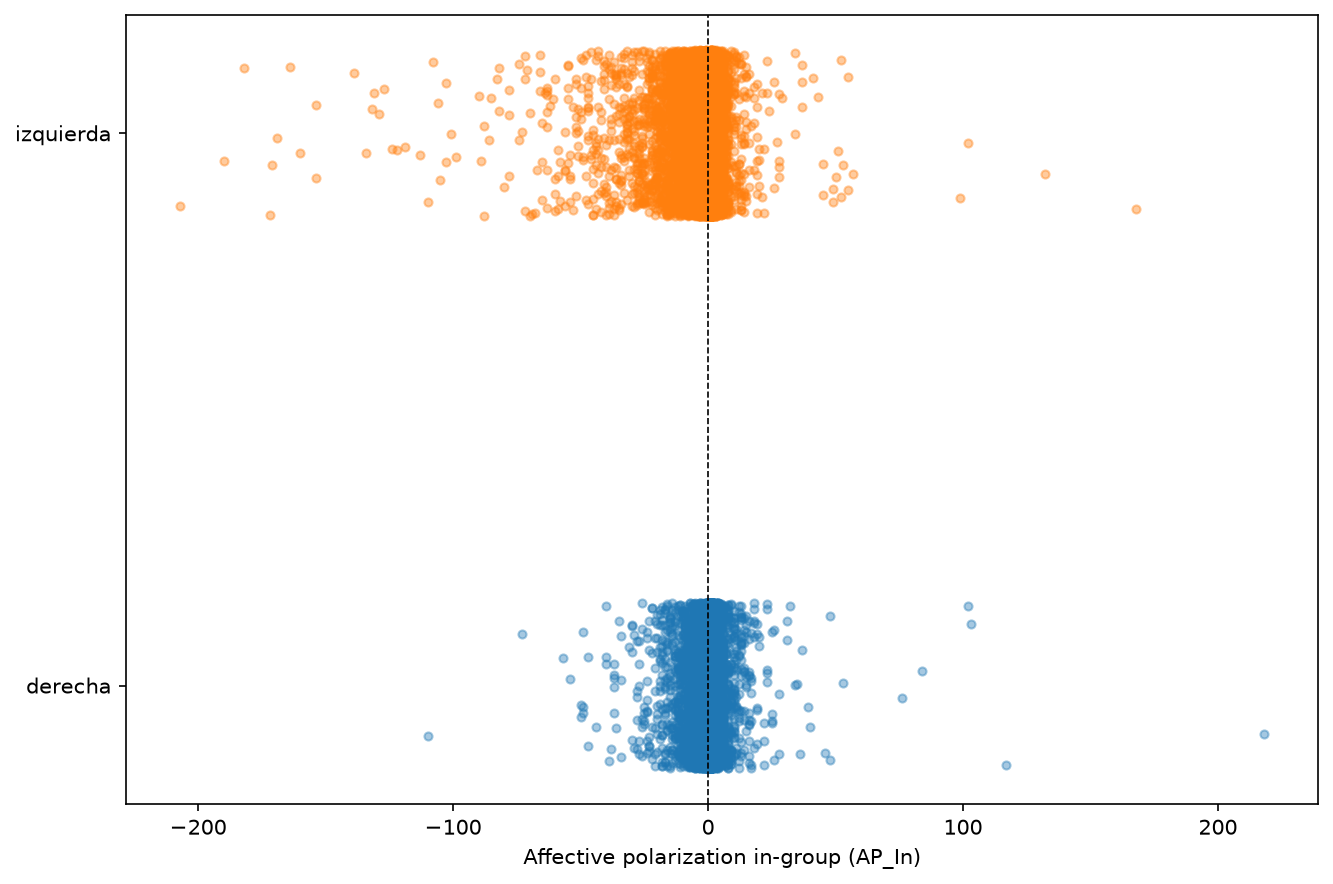
\includegraphics[width=0.98\linewidth]{docs/figures/plot_ap_in.png}
    \caption{Distribución individual de AP$_{In}$ por grupo de afinidad operacional.}
    \label{fig:ap_in}
\end{figure}

\begin{figure}[H]
    \centering
    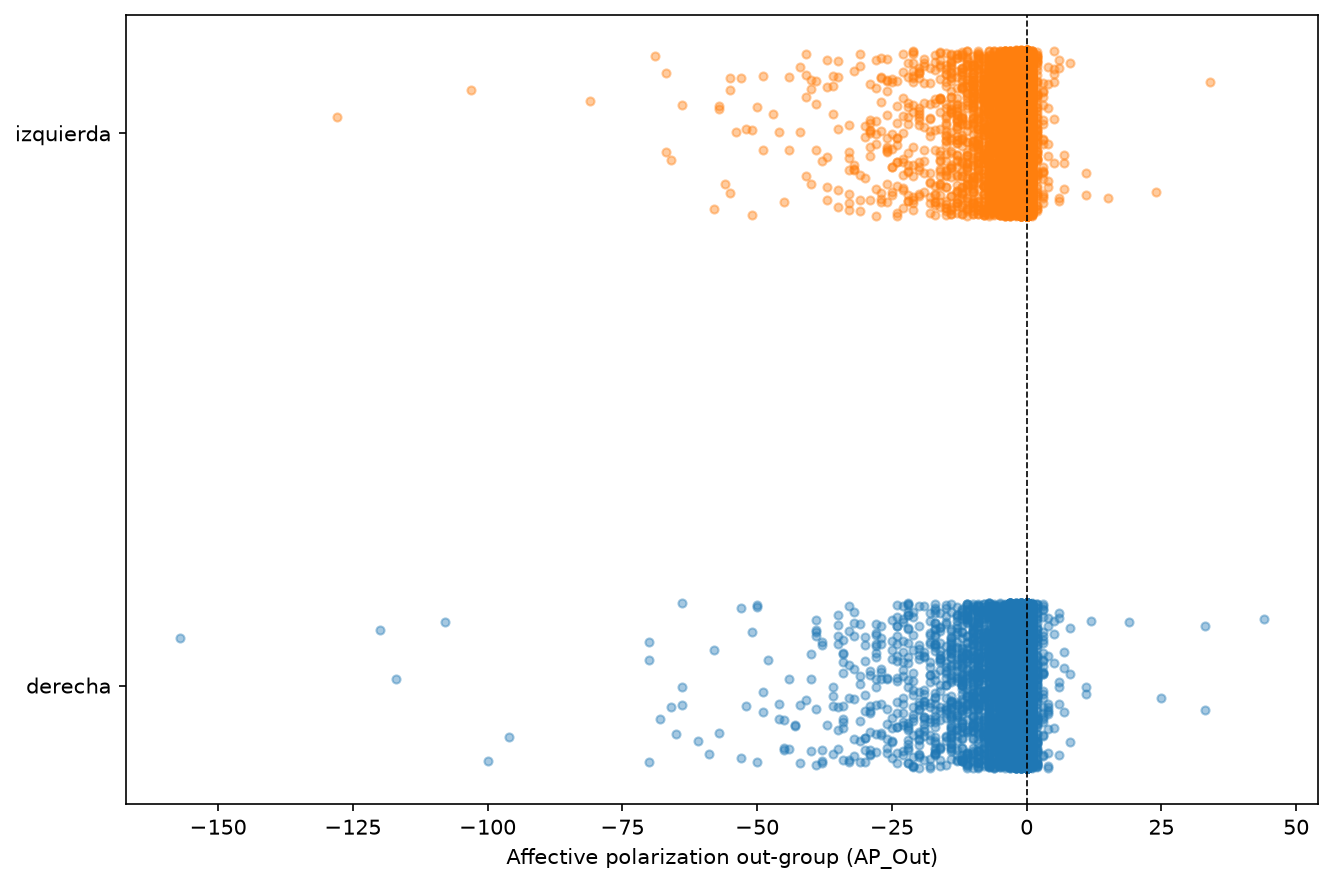
\includegraphics[width=0.98\linewidth]{docs/figures/plot_ap_out.png}
    \caption{Distribución individual de AP$_{Out}$ por grupo de afinidad operacional.}
    \label{fig:ap_out}
\end{figure}

\begin{figure}[H]
    \centering
    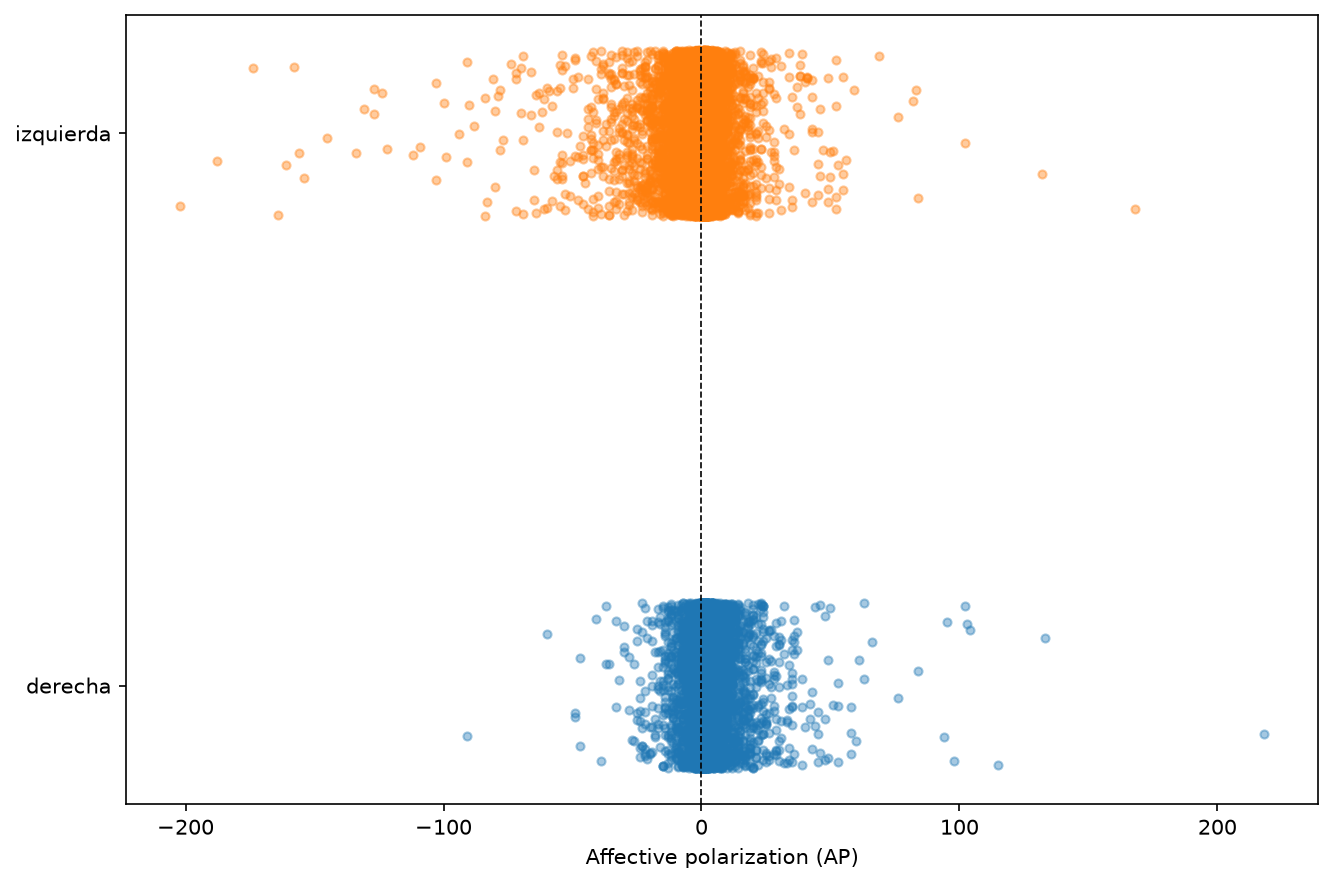
\includegraphics[width=0.98\linewidth]{docs/figures/plot_ap_final.png}
    \caption{Distribución individual de AP por grupo de afinidad operacional.}
    \label{fig:ap}
\end{figure}

\begin{figure}[H]
    \centering
    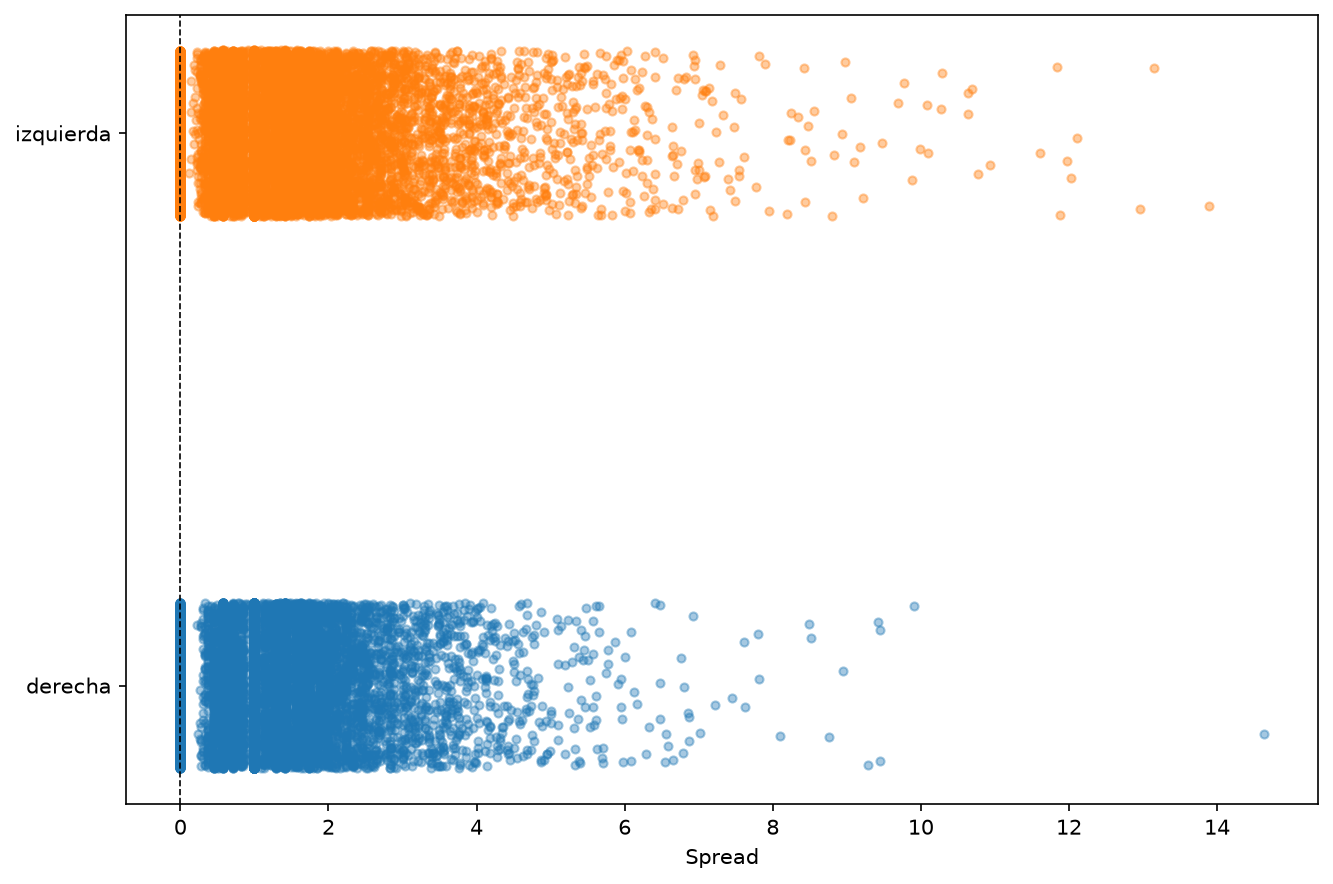
\includegraphics[width=0.98\linewidth]{docs/figures/plot_spread.png}
    \caption{Distribución individual de \textit{spread} por grupo de afinidad operacional.}
    \label{fig:spread}
\end{figure}

El AP medio es positivo para los usuarios asignados a derecha y ligeramente
negativo para los asignados a izquierda. En ambos grupos, AP$_{Out}$ medio es
negativo. Sin embargo, esto no basta para concluir que un grupo manifiesta
mayor polarización afectiva sustantiva: las métricas usan conteos de
sentimiento general como aproximación a interacciones dirigidas a grupos, y
son sensibles al volumen de actividad. Además, el \textit{spread} local usa
como denominador los comentarios positivos y negativos, y no incluye los
neutrales.

El promedio global de AP fue $0.325$ (DE $6.323$) y el de \textit{spread} fue
$1.121$ (DE $0.819$). El elevado porcentaje de usuarios indeterminados también
limita la descripción a quienes aportaron evidencia positiva suficiente para
asignarles un grupo. El universo de usuarios del análisis se forma tras
filtrar comentarios neutrales, por lo que no incluye a quienes solo escribieron
comentarios neutrales.

\subsection{Comparación e interpretación de los resultados}

Al comparar estos patrones con los de Martínez-España et al. \cite{polariz},
el AP$_{In}$ medio del estudio de referencia ($8.662$ para la derecha y
$6.813$ para la izquierda) es positivo en ambos grupos; en esta corrida también
es positivo para derecha ($0.493$), pero negativo para izquierda ($-0.839$).
Los AP medios locales son $1.484$ y $-0.259$, respectivamente, frente a
valores aproximados de $9.885$ y $7.972$ derivados de las tablas del paper.
AP$_{Out}$ medio es negativo en ambos análisis: los valores aproximados del
paper son $-1.223$ para la derecha y $-1.160$ para la izquierda, frente a
$-0.991$ y $-0.580$ en esta corrida. La dirección del resultado coincide,
pero las magnitudes difieren. En conjunto, estos patrones describen resultados
distintos en las métricas observadas, pero no permiten concluir que una
población presente más o menos polarización que la otra.

El \textit{spread} medio local ($1.098$ para derecha y $1.133$ para izquierda)
y la proporción local de nivel alto ($7.12\%$ y $10.21\%$) también son
inferiores a los valores reportados en el paper ($1.874$ y $1.748$; $15.89\%$
y $13.35\%$, respectivamente). Esta diferencia no constituye una comparación
directa: el paper incluye cuatro grupos de Twitter y usa el total de
interacciones como denominador de \textit{spread}, mientras que este análisis
incluye comentarios de YouTube clasificados por fuente, dos grupos políticos
y un pool neutral, y cuenta solo comentarios positivos o negativos en ese
denominador. También difieren las poblaciones, las unidades de análisis y los
umbrales para definir niveles altos. Por ello, las magnitudes y proporciones
no deben interpretarse como un ranking entre estudios ni como una réplica
metodológica.

En conjunto, estos resultados caracterizan sentimiento predicho en los
comentarios observados bajo las fuentes clasificadas y ofrecen métricas
exploratorias de actividad por grupo. No permiten inferir directamente la
postura de cada comentario hacia un actor político, la ideología de sus
autores, la opinión de los votantes ni la polarización afectiva de la
población peruana. Una interpretación más fuerte requeriría validar que la
valencia esté dirigida al objetivo político y examinar la robustez de los
patrones ante la cobertura desigual de canales y el volumen de comentarios.



% \section{Conclusiones y trabajo futuro}

% En este trabajo se aplicó un enfoque simplificado, inspirado en la metodología de
% Martínez-España et al. \cite{polariz}, para analizar el sentimiento político
% expresado en comentarios de TikTok durante la segunda vuelta de las elecciones
% presidenciales peruanas de 2026, utilizando el modelo RoBERTuito sobre un conjunto
% de 2743 comentarios.

% Los resultados evidenciaron un comportamiento consistente con un \textit{echo
% chamber}: las publicaciones asociadas a ambos candidatos registraron favorabilidad
% neta positiva y de magnitud muy similar entre sí, en contraste con el clima
% levemente negativo de las publicaciones neutrales. Esta similitud entre bloques
% políticos, sumada al hecho de que el resultado electoral fue sumamente cerrado,
% refuerza la idea de que el sentimiento expresado en redes sociales debe entenderse
% como un reflejo del clima emocional de la conversación digital, y no como un
% predictor directo de la intención de voto.

% La principal limitación del estudio fue la escasa recurrencia de los usuarios: la
% gran mayoría comentó una única vez y prácticamente ninguno interactuó con
% publicaciones de más de una categoría política. Esto impidió calcular un indicador
% de polarización afectiva individual (\textit{ingroup}/\textit{outgroup}) equivalente
% al de la metodología de referencia \cite{polariz}, restringiendo los resultados a
% una medida de favorabilidad agregada por categoría.

% Como trabajo futuro se plantea ampliar el volumen y la diversidad de las fuentes de
% datos para captar usuarios recurrentes entre distintas orientaciones políticas,
% explorar la detección de menciones a otros candidatos dentro de un mismo comentario
% como señal adicional de polarización, e incorporar una validación manual del modelo
% de clasificación que permita cuantificar su desempeño sobre el dominio específico de
% comentarios políticos en español peruano.

% % conference papers do not normally have an appendix


% % use section* for acknowledgement
% % \section*{Acknowledgment}


% % The authors would like to thank...





% % trigger a \newpage just before the given reference
% % number - used to balance the columns on the last page
% % adjust value as needed - may need to be readjusted if
% % the document is modified later
% %\IEEEtriggeratref{8}
% % The "triggered" command can be changed if desired:
% %\IEEEtriggercmd{\enlargethispage{-5in}}

% % references section

% % can use a bibliography generated by BibTeX as a .bbl file
% % BibTeX documentation can be easily obtained at:
% % http://www.ctan.org/tex-archive/biblio/bibtex/contrib/doc/
% % The IEEEtran BibTeX style support page is at:
% % http://www.michaelshell.org/tex/ieeetran/bibtex/
% %\bibliographystyle{IEEEtran}
% % argument is your BibTeX string definitions and bibliography database(s)
% %\bibliography{IEEEabrv,../bib/paper}
% %
% % <OR> manually copy in the resultant .bbl file
% % set second argument of \begin to the number of references
% % (used to reserve space for the reference number labels box)

\bibliographystyle{IEEEtran}
\bibliography{IEEEabrv, referencies}


\end{document}

